\PassOptionsToPackage{unicode=true}{hyperref} % options for packages loaded elsewhere
\PassOptionsToPackage{hyphens}{url}
%
\documentclass[12pt,]{article}
\usepackage{lmodern}
\usepackage{amssymb,amsmath}
\usepackage{ifxetex,ifluatex}
\usepackage{fixltx2e} % provides \textsubscript
\ifnum 0\ifxetex 1\fi\ifluatex 1\fi=0 % if pdftex
  \usepackage[T1]{fontenc}
  \usepackage[utf8]{inputenc}
  \usepackage{textcomp} % provides euro and other symbols
\else % if luatex or xelatex
  \usepackage{unicode-math}
  \defaultfontfeatures{Ligatures=TeX,Scale=MatchLowercase}
\fi
% use upquote if available, for straight quotes in verbatim environments
\IfFileExists{upquote.sty}{\usepackage{upquote}}{}
% use microtype if available
\IfFileExists{microtype.sty}{%
\usepackage[]{microtype}
\UseMicrotypeSet[protrusion]{basicmath} % disable protrusion for tt fonts
}{}
\IfFileExists{parskip.sty}{%
\usepackage{parskip}
}{% else
\setlength{\parindent}{0pt}
\setlength{\parskip}{6pt plus 2pt minus 1pt}
}
\usepackage{hyperref}
\hypersetup{
            pdftitle={어벤져스},
            pdfauthor={토르 (UNIST); 아이언맨 (Hanyang University)},
            pdfborder={0 0 0},
            breaklinks=true}
\urlstyle{same}  % don't use monospace font for urls
\usepackage{graphicx,grffile}
\makeatletter
\def\maxwidth{\ifdim\Gin@nat@width>\linewidth\linewidth\else\Gin@nat@width\fi}
\def\maxheight{\ifdim\Gin@nat@height>\textheight\textheight\else\Gin@nat@height\fi}
\makeatother
% Scale images if necessary, so that they will not overflow the page
% margins by default, and it is still possible to overwrite the defaults
% using explicit options in \includegraphics[width, height, ...]{}
\setkeys{Gin}{width=\maxwidth,height=\maxheight,keepaspectratio}
\setlength{\emergencystretch}{3em}  % prevent overfull lines
\providecommand{\tightlist}{%
  \setlength{\itemsep}{0pt}\setlength{\parskip}{0pt}}
\setcounter{secnumdepth}{0}
% Redefines (sub)paragraphs to behave more like sections
\ifx\paragraph\undefined\else
\let\oldparagraph\paragraph
\renewcommand{\paragraph}[1]{\oldparagraph{#1}\mbox{}}
\fi
\ifx\subparagraph\undefined\else
\let\oldsubparagraph\subparagraph
\renewcommand{\subparagraph}[1]{\oldsubparagraph{#1}\mbox{}}
\fi

% set default figure placement to htbp
\makeatletter
\def\fps@figure{htbp}
\makeatother

\usepackage{setspace}\doublespacing
\usepackage{fullpage}
\usepackage[utf8]{inputenc}
\usepackage{kotex}
\usepackage{kotex-logo}

\title{어벤져스}
\author{토르 (UNIST) \and 아이언맨 (Hanyang University)}
\date{}

\begin{document}
\maketitle
\begin{abstract}
이 논문은 \ldots{}
\end{abstract}

\setlength{\parindent}{1cm}

\hypertarget{uxc11cuxb860}{%
\section{서론}\label{uxc11cuxb860}}

Bae et al. (2014) 은 분석\ldots{}.

\hypertarget{uxbb38uxd5cc-uxc5f0uxad6c}{%
\section{문헌 연구}\label{uxbb38uxd5cc-uxc5f0uxad6c}}

과거 연구에 \ldots{}

\hypertarget{uxb370uxc774uxd130-uxbc0f-uxc5f0uxad6c-uxbc29uxbc95uxb860}{%
\section{데이터 및 연구
방법론}\label{uxb370uxc774uxd130-uxbc0f-uxc5f0uxad6c-uxbc29uxbc95uxb860}}

데이터는 코스콤, 선형 회귀분석을 사용..

\hypertarget{uxb370uxc774uxd130}{%
\subsection{데이터}\label{uxb370uxc774uxd130}}

서브 섹션

\hypertarget{uxc5f0uxad6c-uxbc29uxbc95uxb860}{%
\subsection{연구 방법론}\label{uxc5f0uxad6c-uxbc29uxbc95uxb860}}

서브 섹션

\begin{center}
<Insert Table 1>
\end{center}

\hypertarget{uxc2e4uxc99d-uxbd84uxc11d-uxacb0uxacfc}{%
\section{실증 분석 결과}\label{uxc2e4uxc99d-uxbd84uxc11d-uxacb0uxacfc}}

연구 결과에 따르면 \ldots{}

\[ r_{t \rightarrow t+k}= \beta_0 + \beta_1 \cdot x_t +\varepsilon_{t \rightarrow k} \]

\hypertarget{uxacb0uxb860}{%
\section{결론}\label{uxacb0uxb860}}

본 논문에서 발견한 \ldots{}

\newpage

\hypertarget{tables-and-figures}{%
\section{Tables and Figures}\label{tables-and-figures}}

한글 논문이라도 Table과 Figure는 영어로 작성하세요.

\begin{table}[!htbp] \centering 
  \caption{} 
  \label{} 
\begin{tabular}{@{\extracolsep{5pt}}lccccccc} 
\\[-1.8ex]\hline 
\hline \\[-1.8ex] 
Statistic & \multicolumn{1}{c}{N} & \multicolumn{1}{c}{Mean} & \multicolumn{1}{c}{St. Dev.} & \multicolumn{1}{c}{Min} & \multicolumn{1}{c}{Pctl(25)} & \multicolumn{1}{c}{Pctl(75)} & \multicolumn{1}{c}{Max} \\ 
\hline \\[-1.8ex] 
rating & 30 & 64.633 & 12.173 & 40 & 58.8 & 71.8 & 85 \\ 
complaints & 30 & 66.600 & 13.315 & 37 & 58.5 & 77 & 90 \\ 
privileges & 30 & 53.133 & 12.235 & 30 & 45 & 62.5 & 83 \\ 
learning & 30 & 56.367 & 11.737 & 34 & 47 & 66.8 & 75 \\ 
raises & 30 & 64.633 & 10.397 & 43 & 58.2 & 71 & 88 \\ 
critical & 30 & 74.767 & 9.895 & 49 & 69.2 & 80 & 92 \\ 
advance & 30 & 42.933 & 10.289 & 25 & 35 & 47.8 & 72 \\ 
\hline \\[-1.8ex] 
\end{tabular} 
\end{table}

\newpage

\begin{figure}
\centering
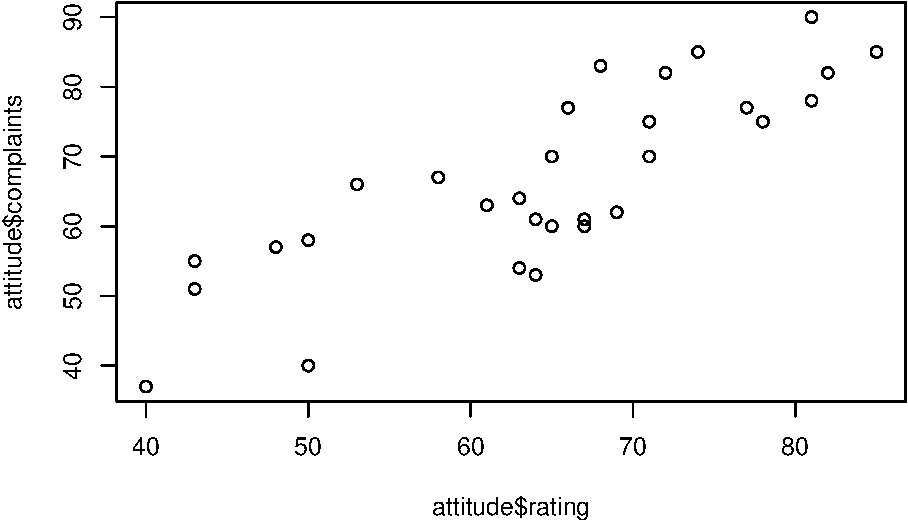
\includegraphics{main_files/figure-latex/unnamed-chunk-2-1.pdf}
\caption{A caption}
\end{figure}

\newpage

\hypertarget{references}{%
\section*{References}\label{references}}
\addcontentsline{toc}{section}{References}

\hypertarget{refs}{}
\leavevmode\hypertarget{ref-bae2014invariance}{}%
Bae, Kyounghun, Albert S Kyle, Eun Jung Lee, and Anna A Obizhaeva. 2014.
``An Invariance Relationship in the Number of Buy-Sell Switching
Points.'' Working Paper, University of Maryland.

\end{document}
